\section{Practical tricks and methods for training}

\begin{frame}{Practical tricks?}
\begin{itemize}
\item There are many practical aspects to be correctly configured to obtain good neural network
based models.
\item You must have already seen many of these concepts in the exercises \& assignments.
\end{itemize}
\end{frame}

\begin{frame}{Model parameter initialization}
\begin{itemize}
\item General principle: initialize with small, random numbers.\\
\codeb{torch.nn.init.normal\_(x, mean=0.0, std=0.01)}, \codeb{torch.nn.init.uniform\_(x, a=-0.1, b=0.1)}
\item More sophisticated methods exist (dependence on input/output dimensions), see e.g.
\begin{itemize}
\item Xavier initializer \codeb{torch.nn.init.xavier\_uniform\_}
\item Variance scaling initializer \codeb{torch.nn.init.kaiming\_uniform\_}
\end{itemize}
\vsp
\item In general: do not overthink, use some standard setups.
\item Except when you want to specify how some model components behave at the beginning of training:
\begin{itemize}
\item e.g. bias initialization for LSTM's forget gate.
\item or when addressing some specific problems...
\end{itemize}
\end{itemize}
\end{frame}

\begin{frame}[fragile]{Model parameter initialization,\\ example}
\begin{python}
def init_weights(m):
    if type(m) == nn.Linear:
        torch.nn.init.xavier_uniform(m.weight)
        m.bias.data.fill_(0.01)

net = nn.Sequential(nn.Linear(2, 2), nn.Linear(2, 2))
net.apply(init_weights)
\end{python}
\vsp
\begin{itemize}
\item Note: \codeb{nn.Sequential} is another way to create a model. 
\item \codeb{.apply} applies the function to all sub-modules.
\item Or do it inside \code{\_\_init\_\_} function of your model.
\end{itemize}
\vsp
\vsp

Have you ever checked how it is done by default in e.g. \codeb{nn.Linear}?
\link{https://pytorch.org/docs/stable/\_modules/torch/nn/modules/linear.html}
\end{frame}

\begin{frame}{Choice of learning rate}
\begin{itemize}
\item Learning rate is typically the most important training hyper-parameter.
\item Different learning rates, different training behaviors.
\item Good strategy: modify learning rate during training.
\end{itemize}
\vsp
\begin{minipage}{0.45\linewidth}
  \begin{center}
    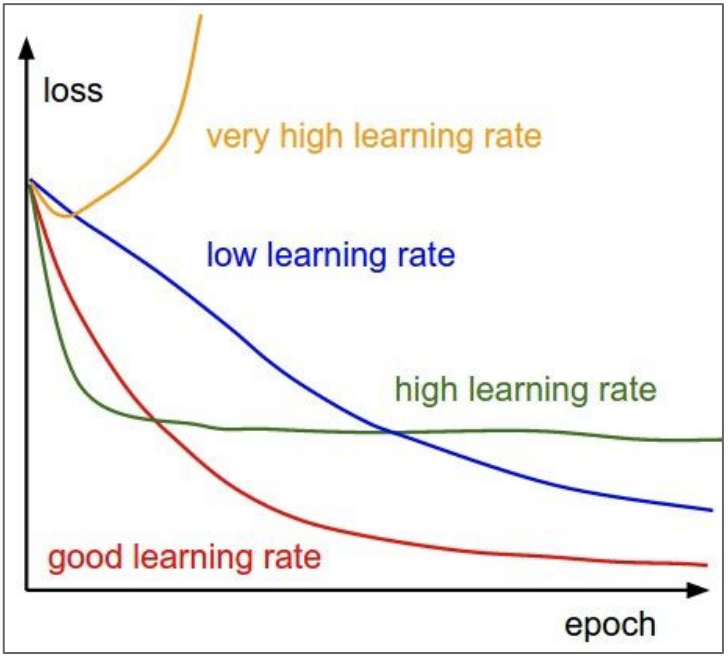
\includegraphics[height=0.6\textheight]{figures/different-lr.png}
  \end{center}
\end{minipage}
\hspace{3mm}
\begin{minipage}{0.45\linewidth}
  \begin{center}
    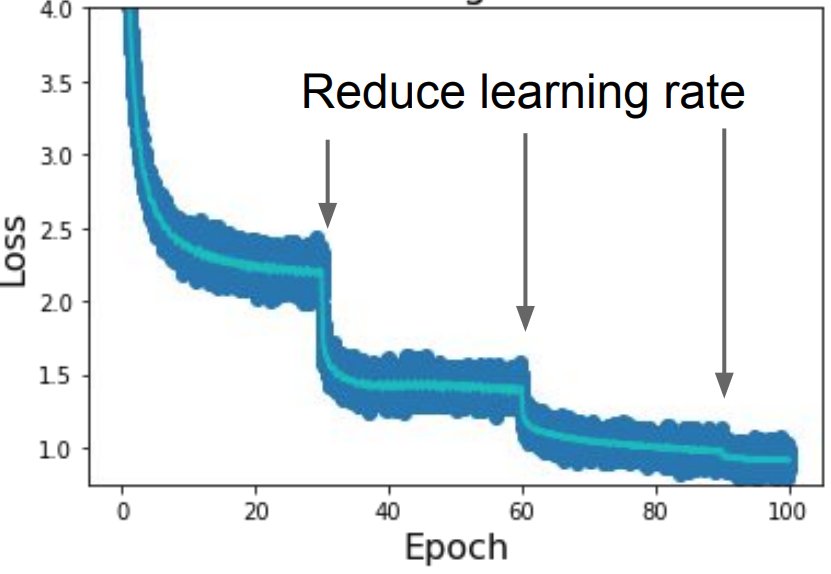
\includegraphics[height=0.6\textheight]{figures/lr-reduce-v2.png}
  \end{center}
\end{minipage}\\
\vspace{5mm}
\scriptsize{Figures taken from \citem{stanford2019training}.}
\end{frame}

\begin{frame}{Learning rate scheduling}
\textbf{How to modify the learning rate during training?}\\
\vspace{5mm}
\begin{minipage}{0.3\linewidth}
  \begin{center}
    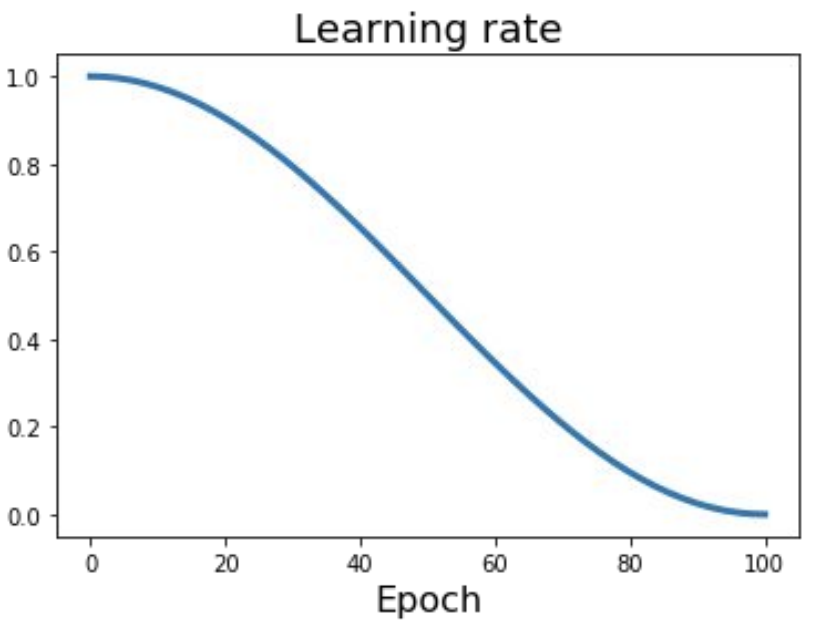
\includegraphics[height=0.35\textheight]{figures/lr-schedule-1.png}
  \end{center}
\end{minipage}
% \hspace{2mm}
\begin{minipage}{0.3\linewidth}
  \begin{center}
    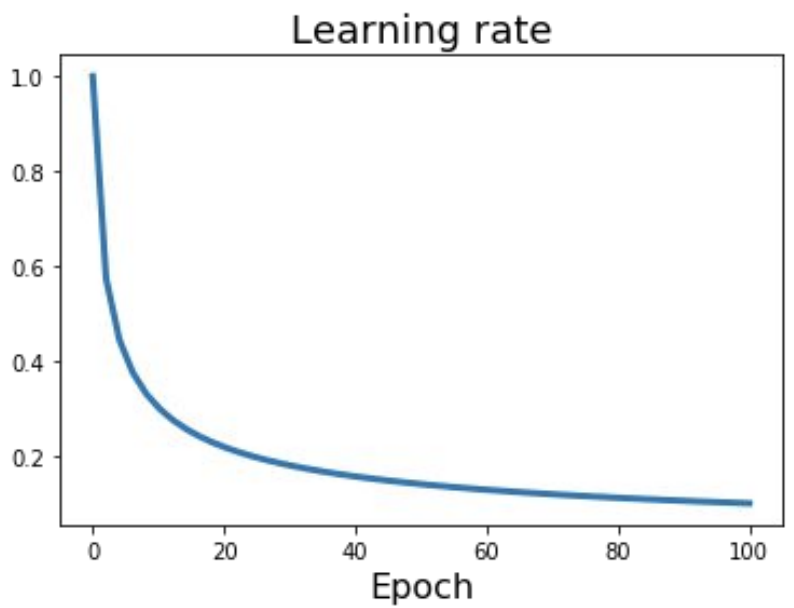
\includegraphics[height=0.35\textheight]{figures/lr-schedule-2.png}
  \end{center}

\end{minipage}
% \hspace{1mm}
\begin{minipage}{0.3\linewidth}
  \begin{center}
    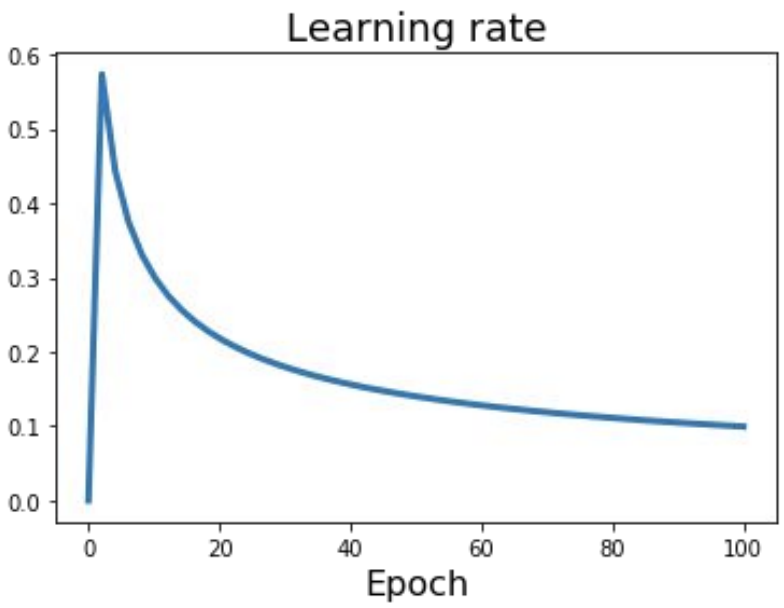
\includegraphics[height=0.35\textheight]{figures/lr-schedule-3.png}
  \end{center}
\end{minipage}\\
\vspace{5mm}
{\scriptsize Figures taken from \citem{stanford2019training}.}

\begin{itemize}
\item Or better: change dependent on performance on the \textbf{validation set}.
\item If improvement on the validation set is less than $x$\%, then reduce the learning rate by some factor.
\end{itemize}
\end{frame}

\begin{frame}[fragile]{Learning rate scheduling,\\example}
\begin{itemize}
\item \codeb{torch.optim.lr\_scheduler} provides different strategies.\\
\codeb{ReduceLROnPlateau}, \codeb{CosineAnnealingLR}, ...
\end{itemize}
\begin{python}
optimizer = torch.optim.SGD(model.parameters(), lr=0.1, momentum=0.9)
scheduler =
    torch.optim.lr_scheduler.ReduceLROnPlateau(optimizer, 'min')

for epoch in range(10):
     train(...)
     val_loss = validate(...)
     # Note that step should be called after validate()
     scheduler.step(val_loss)
\end{python}
\end{frame}

\begin{frame}{Depending on optimizers}
\begin{itemize}
\item The range of good choice of initial learning rate depends on the optimizer.
\item Common optimizers: SGD and Adam.
\item Typical configurations/heuristics:
\item[-] SGD: rather high learning rate (e.g. \texttt{1}, \texttt{0.1}) typically with gradient clipping (next page).
\item[-] Adam: rather small learning rate (e.g. \texttt{1e-3}, \texttt{1e-4}).
\end{itemize}
Also Adam often requires none or only some minimum learning rate scheduling.
\end{frame}


\begin{frame}[fragile]{Other training helper tricks}
Techniques to \emphbf{stabilize training}, allowing us to use \textbf{high learning rates} without getting the model to crash (\texttt{NaN} loss value):
\vsp
\begin{itemize}
\item \emphbf{Gradient clipping}
\begin{itemize}
\item There are a couple of ways to do it.
\item Common approach: global norm clipping.
\item[-] One hyper-parameter: max gradient norm $M$.
\item[-] If norm computed over all gradients is larger than $M$, scale all gradients by $M$/norm.
\end{itemize}
\end{itemize}
\begin{python}
clip_val = 1.0

loss.backward()
torch.nn.utils.clip_grad_norm_(model.parameters(), clip_val)
optimizer.step()
\end{python}
\end{frame}

\begin{frame}[fragile]{Other training helper tricks (cont'd)}
\begin{itemize}
\item \emphbf{Normalization layers}: transform input $x$ to $y$ via:
\[
y = \dfrac{x-\E[x]}{\sqrt{\Var[x]}} * a + b
\]
where $a$ and $b$ are vectors and learnable parameters.\\
Different methods depending on the support of computing mean $\E[x]$ and variance $\Var[x]$:
\vsp
\item \emphbf{Layer normalization}: 
\begin{itemize}
\item mean and variance computed along the \textbf{feature dimension}.
\end{itemize}
\item \emphbf{Batch normalization}
\begin{itemize}
\item mean and variance computed per-dimension over the \textbf{mini-batches}.
\item during training: keeps updating estimates of its computed mean and variance, which are then used during evaluation.
\end{itemize}
\end{itemize}
\end{frame}

\begin{frame}{Choosing model hyper-parameters}
\begin{itemize}
\item \textbf{Possible strategy}: put as many parameters as possible, until the model overfits.
\item Apply \emphbf{regularization techniques} to be able to make it even larger.
\item Also: if larger dataset (or data augmentation), then larger model size.
\end{itemize}
\end{frame}

\begin{frame}{Overfitting \& Early stopping}
\vspace{-3mm}
\begin{itemize}
\item When your setups are correct, and the model has \emphbf{enough capacity} (large enough number of parameters), your model should get very good performance on the \textbf{training data} when trained for long.
\item Typically, performance on validation set degrades at some point (again, if model is large enough!): model \emphbf{overfits} to training data.
\item Good strategy: \emphbf{stop training earlier, by checking validation error}.
\end{itemize}
\begin{figure}
\hspace{-10mm}
                        \centering
                        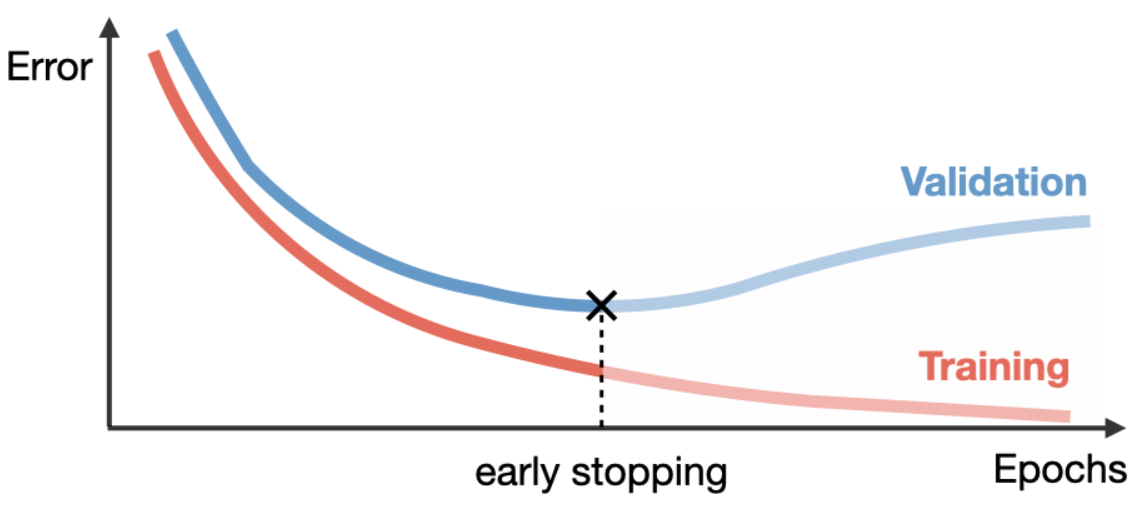
\includegraphics[width=.7\linewidth]{./figures/overfit.png}
\end{figure}
\scriptsize{Figure taken from \citem{stanford2019cheat}.}
\end{frame}

\begin{frame}[fragile]{Regularization methods}

\begin{itemize}
\item Standard machine learning regularization techniques can be applied to neural networks.
\item Extra penalty loss on the weights: minimize its L1, L2 norms...
\item In PyTorch, all standard optimizer has an option for \textit{weight decay}:
\end{itemize}
\begin{python}
optimizer = torch.optim.SGD(
    model.params(), lr=0.01, weight_decay=1e-4)
\end{python}
\begin{itemize}
\item which is equivalent to L2 regularization for many optimizers (not for Adam).
\item Extra training hyper-parameter...
\end{itemize}
\end{frame}

\begin{frame}{Dropout}
\vspace{-5mm}
\begin{itemize}
\item Popular regularization methods for neural networks: \emphbf{dropout}.
  \begin{center}
    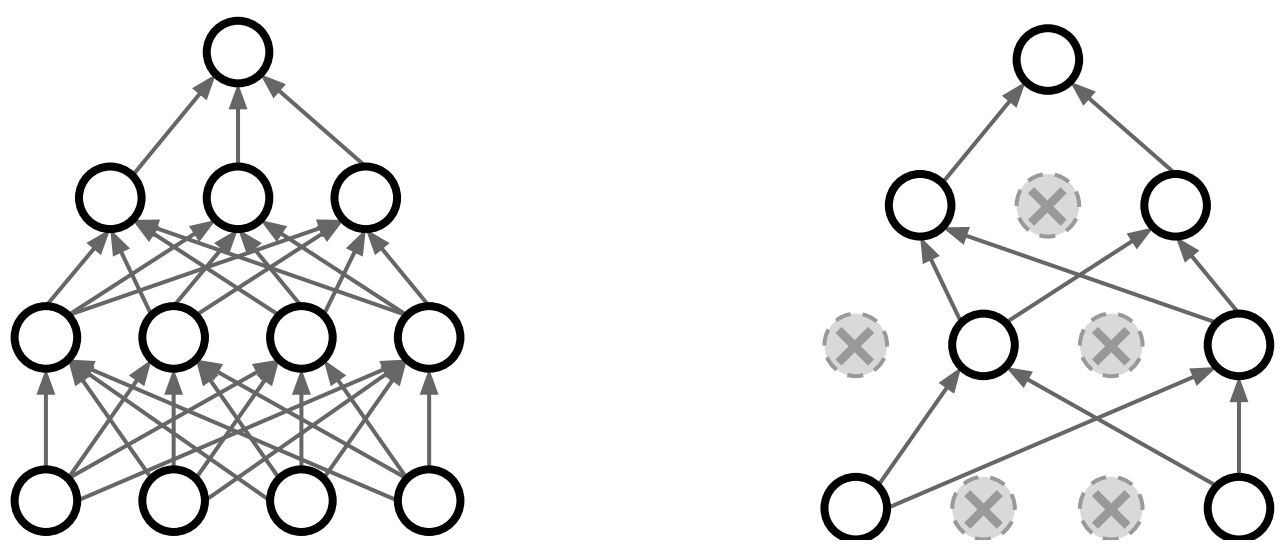
\includegraphics[height=0.4\textheight]{figures/dropout.png}
  \end{center}
\vspace{-3mm}
{\tiny Figure taken from \cite{stanford2019training}.}
\item One hyper-parameter: dropout rate $p$.
\item Set each activation to 0 with a probability of $p$ during training.
\item At test time: use all activations but scale by $1-p$.
\item (Or scale by $1/(1-p)$ during training instead, and do nothing at test time).
\item Note: introduce different model behaviors between train and eval. PyTorch reminder: \codeb{mode.train()} and \codeb{model.eval()}.
\end{itemize}
\end{frame}

\begin{frame}[fragile]{Dropout, implementations}
\begin{itemize}
\item Dropout can be defined just as a regular layer:
\begin{python}
>>> input = torch.randn(2, 6)
>>> m = nn.Dropout(p=0.5)
>>> output = m(input)
>>> input
tensor([[-0.0863,  0.6893,  0.0138, -2.0447,  1.1345,  0.3555],
        [ 1.1229,  0.0027,  0.0993, -0.7476,  0.5680, -0.4255]])
>>> output
tensor([[-0.1726,  1.3785,  0.0276, -0.0000,  2.2689,  0.7110],
        [ 0.0000,  0.0054,  0.1985, -1.4953,  1.1359, -0.0000]])
\end{python}
\item Note: some Pytorch build-in layers/modules already have an internal dropout option.
\end{itemize}
\begin{python}
\end{python}
\end{frame}

\begin{frame}{Model averaging, for evaluation}
\begin{itemize}
\item \emphbf{Ensembling}: combine multiple models' output distributions for \textbf{evaluation}.\\
e.g. combination by weighted averaging.\\
Model combinations should never hurt! 
\item \emphbf{Model averaging}: average weights of different models with the same architecture.\\
In some cases helpful to average different model checkpoints in the same training run (relation to some special optimization algorithm...).
\end{itemize}
\end{frame}

% \begin{frame}{Summary}
% \textbf{What have we learned?}
% \begin{itemize}
% \item Practical tricks to make training to work.
% \begin{itemize}
% \item overfitting/early stopping
% \item how to choose learning rate?
% \item how to modify learning rate during training?
% \item how to stabilize training?
% \item how to tune model hyper-parameters?
% \item dropout
% \item model averaging
% \end{itemize}
% \end{itemize}
% \vsp
% \textbf{Coming up next...}
% \begin{itemize}
% \item Summary of the course.
% \item ...
% \end{itemize}
% \end{frame}

% \section{Summary: general recipe}
% \begin{frame}{Specifying model}
% \textbf{Typical model hyper-parameters:}
% \begin{itemize}
% \item Number of layers
% \item Size of hidden layers
% \item ...
% \end{itemize}
% \end{frame}
% 
% \begin{frame}{Setting up training}
% \textbf{Engineering choices to be made.}
% \textbf{Setting up optimizer:}
% \begin{itemize}
% \item Optimizer (SGD, Adam, Adagrad)
% \item Initial learning rate
% \item Learning rate reducing strategy
% \item Gradient clipping.
% \item Stopping criteria.
% \end{itemize}
% \vsp
% \textbf{Batch construction details}:
% \begin{itemize}
% \item Batch size
% \item (for sequence models): maximum sequence length?
% \item Some special shuffling after each epoch?
% \end{itemize}
% \end{frame}